\chapter{Bite Size Case Studies For Systems-Based Public Health Practice}
\openepigraph{%
I employ case studies of failure into my courses, emphasizing that they teach us much more than studies of success. It is not that success stories cannot serve as models of good design or as exemplars of creative engineering. They can do that, but they cannot teach us how close to failure they are.
}{Henry Petroski}

\marginnote{
		\newthought{Key Message:} Public Health Intelligence is not going to become more effective through systems thinking if it doesn't begin to document some of it's steps along this journey. Here are a few of my first steps. Some are failures, but most are just incomplete -- neither complete failures nor complete successes. Learnings.
}


\section*{Introduction}
The case studies presented in this chapter were derived from work that I have participated in, either through my employment in public health or through one of my 'passion projects'. While they don't always fall neatly into the crisp categories (because they can and will be used together): Systems thinking, futures thinking, and systems modelling best aligns with how I think about these approaches.

\section{Incorporating New Knowledge Using A Systems-Based Approach}
\begin{description}
	\item[What?] A trans-disciplinary effort to understand the role of environmental microbiomes was initiated through a series of systems thinking workshops that resulted in a Health Urban Microbiome Initiative that is encapsulated in the ‘HUMI’ causal loop diagram (Figure~\ref{fig:humi}).
	\item[Why?] A number of instigating researchers (public health, restoration ecology and immunology) wanted to develop a large research effort around the idea that there urban populations were largely not exposed to ‘healthy urban microbiomes’ and therefore their rate of immune dysfunction was increasing rapidly around the globe.
	\item[So what?] Futures thinking meets systems thinking. A large number of researchers, many internationally recognised for world class research, believe that emerging field of microbiome science will have a huge impact on public health thinking, particularly around health improvement through exposure to biodiverse green spaces that have healthy microbiomes that in turn could reduce population scale immune dysfunction and associated chronic disease.
	\item[Insight?] Biodiversity loss, growth of urban populations and immune dysfunction are interlinked, and the loss of environmental microbial diversity may be responsible. Restoration of environmental microbiomes may improve population health globally.
\end{description}

\begin{figure*}[h]
	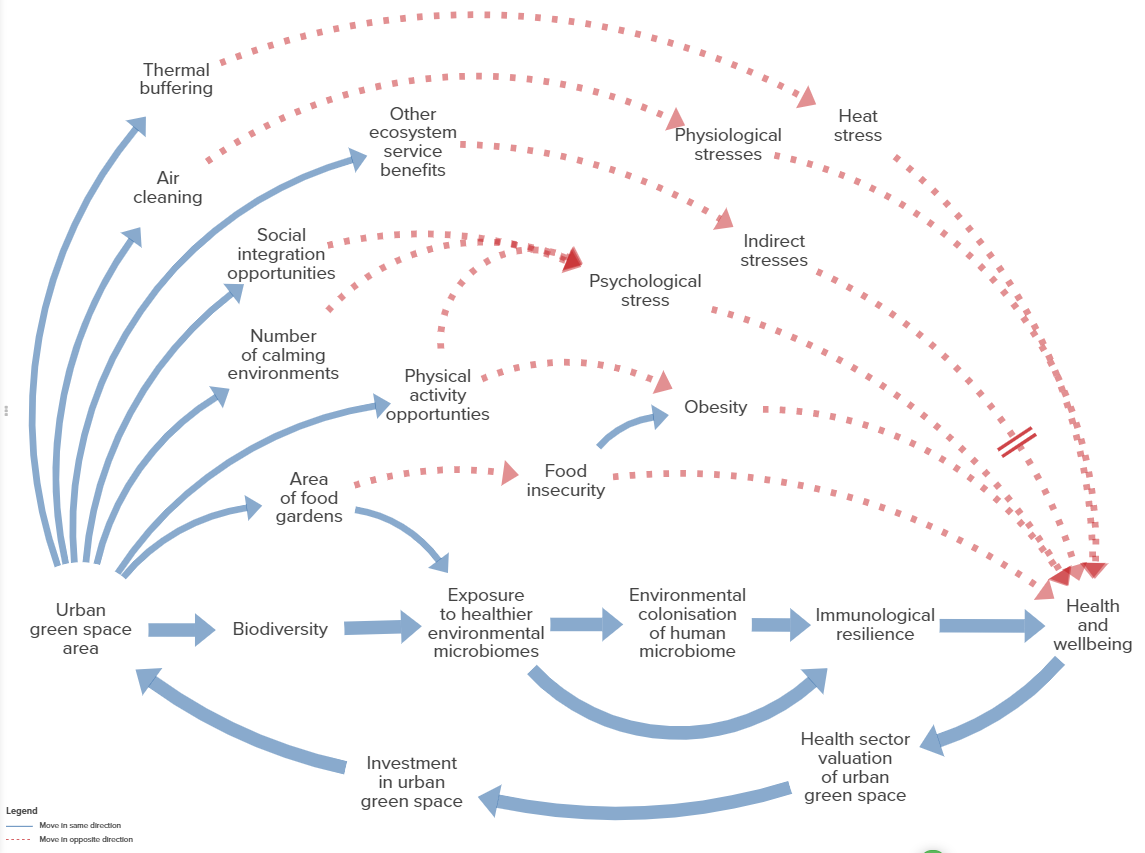
\includegraphics[width=\linewidth]{./figures/HUMI.png}
	\caption[Healthy Urban Microbiome Initiative][6pt]{Causal loop diagram pulled together through extensive consultation with a large group of Australian researchers in Adelaide (Source~\href{https://kumu.io/chrisskelly/humi}{Kumu}).}
	\label{fig:humi}
\end{figure*}



\section{Social Network Modelling for Outbreak Response}
\begin{description}
	\item[What?] Multi-dataset visualisation of potential transmission networks in the Dorset system using a Kumu.io. These visualisations are updated every day and processed using Python scripts (Figure~\ref{fig:socialnetwork}).
	\item[Why?] So that analysts could spend more time looking for insights and less time managing spreadsheets and other data sets in order to support local contact tracing and settings assessment.
	\item[So what?] Reduces analyst time and cost, improves speed of data processing and aids insight development and sharing.
	\item[Insight?] Even 10,000+ data elements and relationships can be explored in minutes in this form and it demonstrates how we can truly extract value from working more closely with Local Public Health Intelligence. PHE data sets, merged with local data sets and explored in KUMU.io after formatting. Almost all of this processing done without analyst intervention.
\end{description}

\begin{figure*}[h]
	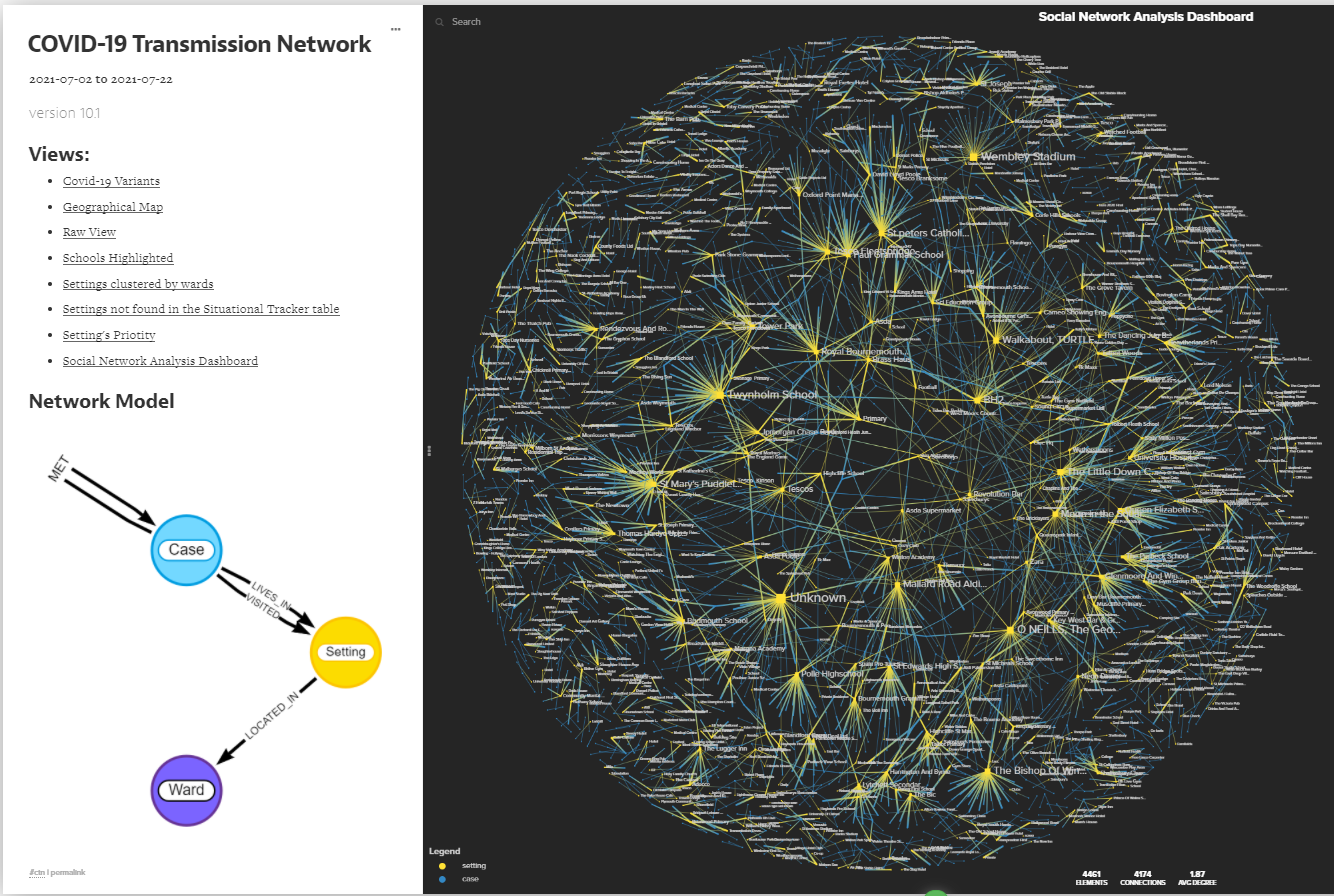
\includegraphics[width=\linewidth]{./figures/Covid19 Social Networks.png}
	\caption[Double Diamond Design Process][6pt]{This is the interface of my copy of a Covid-19 SEIR (Susceptible-Exposed-Infected-Recovered) model developed for Public Health Dorset by (Source~\href{https://www.tanzo.org/}{Tanzo Creative} (Source~\href{https://insightmaker.com/insight/3aozzaFwITwi2Cn6ewR5Wj/Clone-of-Infectious-Disease-Model-Version-4-0}{Insight Maker}). \newthought{Must clear with SC -- PHD DPH Before sharing}Covid-19 Transmission Network (No link as this is sensitive data, but demonstration of site possible with site owner permission).}
	\label{fig:socialnetwork}
\end{figure*}


\section{Systems-Based Healthy Places Scenario Planning}

\begin{description}
	\item[What?] Workshop with senior leaders from across the Dorset health system to identify strategies to take Dorset towards a future of ‘healthy places’
	\item[Why?] Dorset is already seen as wonderful and beautiful landscape that people want to live, work and visit in. However, rarely to people from all walks of the health system consider its health giving potential.
	\item[So what?] Environment is a key component of the ‘wider determinants of health. In the context of health improvement, Dorset’s health places can be viewed as health assets.
	\item[Insight?] The highest ranked strategy for using Dorset’s ‘green’ assets for health improvement was to align population health priorities with political priorities.
\end{description}

\href{https://www.publichealthdorset.org.uk/blogs/the-future-of-healthy-places-developing-futures-strategies.aspx}{The future of ‘healthy places’ — Developing futures strategies}

Is it possible for a group of colleagues to get together, develop a vision of what we want our future to look like AND then actually develop strategies to work towards it?

(Table~\ref{tab:contrasting}).

\begin{table}[h]
	%\resizebox{\textwidth}{!}{
	\begin{center}
		\footnotesize%
		\begin{tabularx}{\linewidth}{p{0.04\linewidth} p{0.135\linewidth} p{0.275\linewidth} p{0.045\linewidth} p{0.35\linewidth}}
			\toprule
			Rank & Focus & Proposed Strategy & Votes & Relevant Work Underway \\
			\midrule
			\multirow{2}{*}{1} & \multirow{2}{\hsize}{Political priorities} & \multirow{2}{\hsize}{Align population health and political priorities} & \multirow{2}{*}{24} & Systems working approach\vspace{0.5\baselineskip} \\
			& & & & Narrative capacity developed with local university media faculty input\vspace{\baselineskip}\\
			
			\multirow{3}{*}{2} & \multirow{3}{\hsize}{Natural Environments} & \multirow{3}{\hsize}{Maximise opportunities from natural environments in local spaces by evaluating health impacts} & \multirow{3}{*}{16} & Public health programme evaluation effort\vspace{0.5\baselineskip} \\
			& & & & System working approach\vspace{0.5\baselineskip} \\
			& & & & Healthy places programme\vspace{\baselineskip} \\
			
			\multirow{2}{*}{3} & \multirow{2}{\hsize}{Active Travel} & \multirow{2}{\hsize}{Increase active travel opportunities as a key element of all travel planning} & \multirow{2}{*}{13} & Systems working approach\vspace{0.5\baselineskip} \\
			& & & & Quantifying accessibility to green space project\vspace{\baselineskip} \\

			\multirow{2}{*}{4} & \multirow{2}{\hsize}{Volunteer resource} & \multirow{2}{\hsize}{Older population is a rich source of skill and experience that could become a major volunteer resource} & \multirow{2}{*}{12} & Prevention at scale – aging well programme\vspace{0.5\baselineskip} \\			
			& & & & System working approach\vspace{0.5\baselineskip} \\
			& & & & Locality working programme\vspace{0.5\baselineskip} \\
			& & & & Health Champions Project\vspace{\baselineskip} \\

			\multirow{2}{*}{4} & \multirow{2}{\hsize}{Sustainable building strategy} & \multirow{2}{\hsize}{Develop a sustainable building strategy (Healthy green developments in partnership)} & \multirow{2}{*}{12} & Healthy places programme\vspace{0.5\baselineskip} \\			
			& & & & Spatial planning development project\vspace{0.5\baselineskip} \\
			& & & & System working approach\vspace{0.5\baselineskip} \\

			\bottomrule
		\end{tabularx}
	\end{center}
	\caption{A subset of the top proposed strategies that senior leaders within the Dorset health system identified during a day-long workshop – a first introduction to futures thinking for the vast majority of participants.}
	\label{tab:contrasting}
\end{table}

\section{Systems-Based Horizon Scanning With Machine Learning Tools}

\begin{description}
	\item[What?] The use of ShapingTomorrow’s AI to scan the horizon has radically changed the process and effort required for organisations to identify trends and weak signals. Public Health Dorset created its own ShapingTomorrow website (Figure~\ref{fig:shapingtomorrow}).
	\item[Why?] There were a number of futures thinking projects that the analyst team felt would contribute to the intelligence and insight programme.
	\item[So what?] With a relatively small team, it was impossible to dedicate the resources to horizon scanning that were needed to be able to produce regular reporting. With AI – horizon scanning is within reach.
	\item[Insight?] Combining horizon scanning with AI and associated data analytics might be a game changer in terms of facilitating more meaningful futures thinking in organisations.
\end{description}

The Future of Healthy Places — a first glimpse…

Are you interested in working towards a future that has healthier places to live, work and learn? If you are, read on. We are using futures studies methods to envision what that future might look like, and my colleagues and I will use this blog to share our insights.

The future of Healthy Places -- Urban Green Space

The first point to make is that research examining the relationship between proximity to well managed urban green space and good health is very consistent – green space in urban environments benefits a population’s health in multiple ways. Not just in urban environments, that’s what we are interested in here, but natural landscapes provide essential ecosystem services from catchment level through to global scale services. Nature is good. Many of us like to wander in green fields and forests when we get the chance – it makes us feel good. Most people get that, but there’s more.

The future of ‘healthy places’ -- Global Warming and Population Ageing

This is a ‘futures’ story about Global Warming and Population Ageing, two global mega trends, and their likely impact Across Dorset, Bournemouth and Poole. We took a small peak into the future and this is what we saw.

\begin{figure*}[h]
	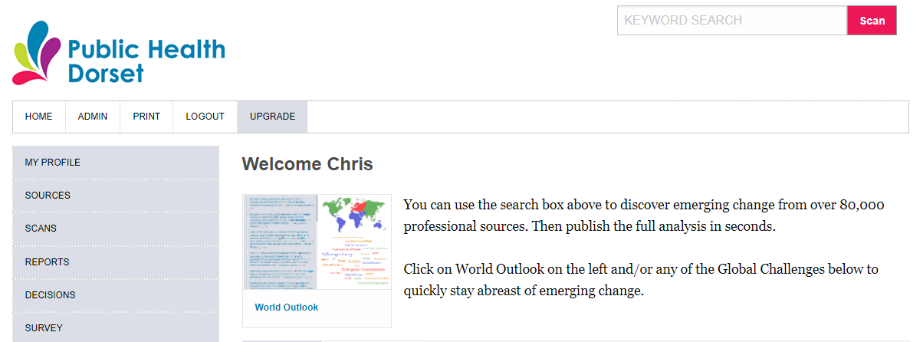
\includegraphics[width=\linewidth]{./figures/ShapingTomorrow.png}
	\caption[Shaping Tomorrow][6pt]{Shaping Tomorrow is an AI horizon scanning tool used to identify what the experts are saying about the future  (\href{https://shapingtomorrow.com}{Shaping Tomorrow Maker}).}
	\label{fig:shapingtomorrow}
\end{figure*}


\section{Imagining A New More Resilient Public Health}
\begin{description}
	\item[What?] The UNFCCC set up a new programme called Resilience Frontiers in 2019 with the express purpose to create “disruption” around how we think about the future of climate change adaptation.
	\item[Why?] Time is running out. The climate emergency is upon us, climate mitigation is not working, and we will be unable to avoid major, maybe catastrophic climatic changes. New thinking is required.
	\item[So what?] They have created eight pathways through which to focus thinking, innovation and the development of new adaptions strategies. Pathway 6. Optimising future health and wellbeing using a holistic and ecosystem approach [Pathway Lead is Dr Chris Skelly, UK]. This is health improvement.
	\item[Insight?] description
\end{description}

Resilience Frontiers was initiated at the Songdo, South Korean futuring event and I wrote a blog a day over the 5-day event, setting out the approach taken at this event.

Resilience Frontiers: Day 1 — Probable Futures. I’m participating in a United Nations Framework Convention on Climate Change (UNFCCC) sponsored event in Song-do, South Korea this week. As part of a larger event on Adaptation to Climate Change, this Resilience Frontiers event, is a five day futuring…

Resilience Frontiers: Day 2 — Desired Futures. Sounds like a population health challenge! The day began with a restatement of the challenge involved in building resilience in the face of climate change; it will be a very familiar problem to those of you working in Public Health…

Resilience Frontiers: Day 3 — Strange Futures. “Never doubt that a small group of thoughtful, committed citizens can change the world; indeed, it’s the only thing that ever has.” Margret Mead Day 1 — Probable Futures — identify and describe what we think is most likely…

Resilience Frontiers: Day 4 — Group Moonshot. We had an incredibly long day today or so it seemed. Group work is exhausting, but satisfying when the discussions are interesting and complex. We followed the same process for making a Moonshot as we did on Day 2…

Resilience Frontiers: Day 5 — Conceiving Policy. Thoughts on the Week This was a long and often intense week — as only these types of events can be. The reality of actually gathering together 125 people from a variety of professional, cultural and demographic backgrounds…

Resilience Frontiers 2021-2030

Each of the eight RF Pathways are to chart their own way through the development of new ideas and the development of innovative adaption projects and strategies.


\section{Public Health Intervention Planning Tool}
\begin{description}
	\item[What?] A generic intervention planning tool for public health colleagues. Captures the dynamics of any intervention based on three critical elements: intervention reach, intervention compliance and intervention efficacy. It allows local systems to tailor costs and population to their situation (Figure~\ref{fig:intervention}).
	\item[Why?] There seems to be a wide-spread lack of appreciation amongst public health colleagues on the value of using these three elements in the management and evaluation of intervention programmes.
	\item[So what?] Knowledge to action. If we want to improve public health interventions, we must develop a better shared-understanding of why some interventions are more successful than others.
	\item[Insight?] High efficacy interventions do not necessarily make the best public health interventions. ‘Reach’ and ‘compliance’ are intervention elements that are determined by the health system and its users, and we need to actively incorporate this into our knowledge to action work.
\end{description}

\marginnote{Blog: \href{https://www.publichealthdorset.org.uk/blogs/future-of-public-health-intervention-three-cold-hard-numbers.aspx}{Future of Public Health Intervention: Three Cold Hard Numbers}
}

People are full of ideas, but how do we harness discussions about population health interventions and move them rapidly into real-world thinking and planning.

\begin{figure*}[h]
	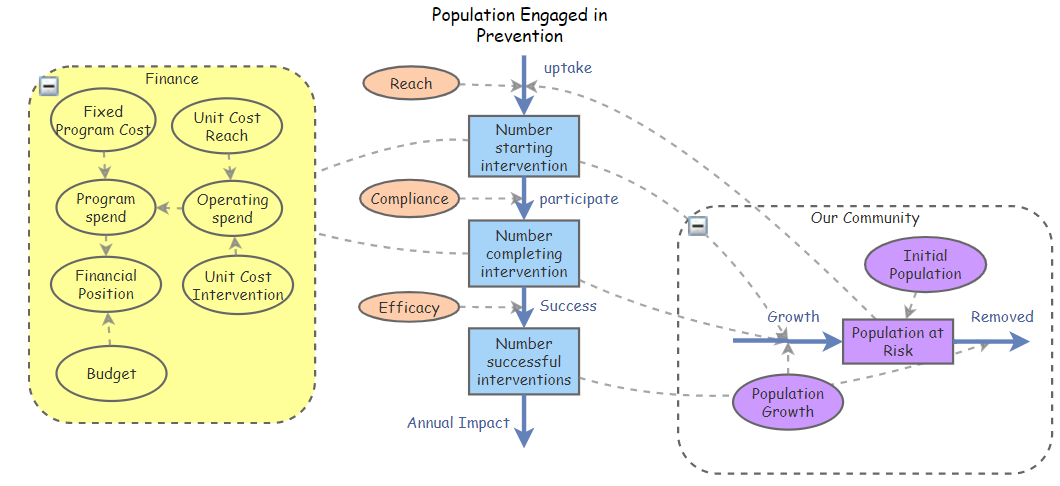
\includegraphics[width=\linewidth]{./figures/Intervention Planning Tool.png}
	\caption[Double Diamond Design Process][6pt]{This is the interface of my copy of a CVD Prevention Model that I modified from a model developed  after~\href{https://www.tanzo.org/}{Tanzo Creative} (\href{https://insightmaker.com/insight/1Oqiscp4ZdbYBaElk4Qq9W/CVD-System-Dynamics-Model-V1-1}{Insight Maker}).}
	\label{fig:intervention}
\end{figure*}


\section{Covid-19 Response Decision-Making}

\begin{description}
	\item[What?] In April 2020 Dorset Public Health commissioned a systems model to capture what was known about SARS-CoV-2 community transmission in order to be able to simulate the Dorset situation (Figure ~\ref{fig:seir}).
	\item[Why?] There is very little epidemiological knowledge within the Dorset system, especially in infectious disease. We believe the model as a reservoir of what we know and understand about the nature of this disease, would be an engaging tool to develop a better shared-understanding.
	\item[So what?] Knowledge to action. We will be conducting a post-hoc evaluation, but I feel that introducing this model into the Dorset ICS’s ‘Covid-19 epicell’ improved the quality of discussion, which in turn improved decision-making. This was our objective and we will attempt to evaluate this later in the year.
	\item[Insight?] Providing colleagues with recent trend data (deaths, cases, hospitalisations) provoked the question – “so what will happen next?” Providing colleagues with a model projection provoked the question – “how do we know this is right?” The first response takes us to more data. The second response takes us straight into a conversation about the dynamics of Covid-19 in our community.
\end{description}

\begin{figure*}[h]
	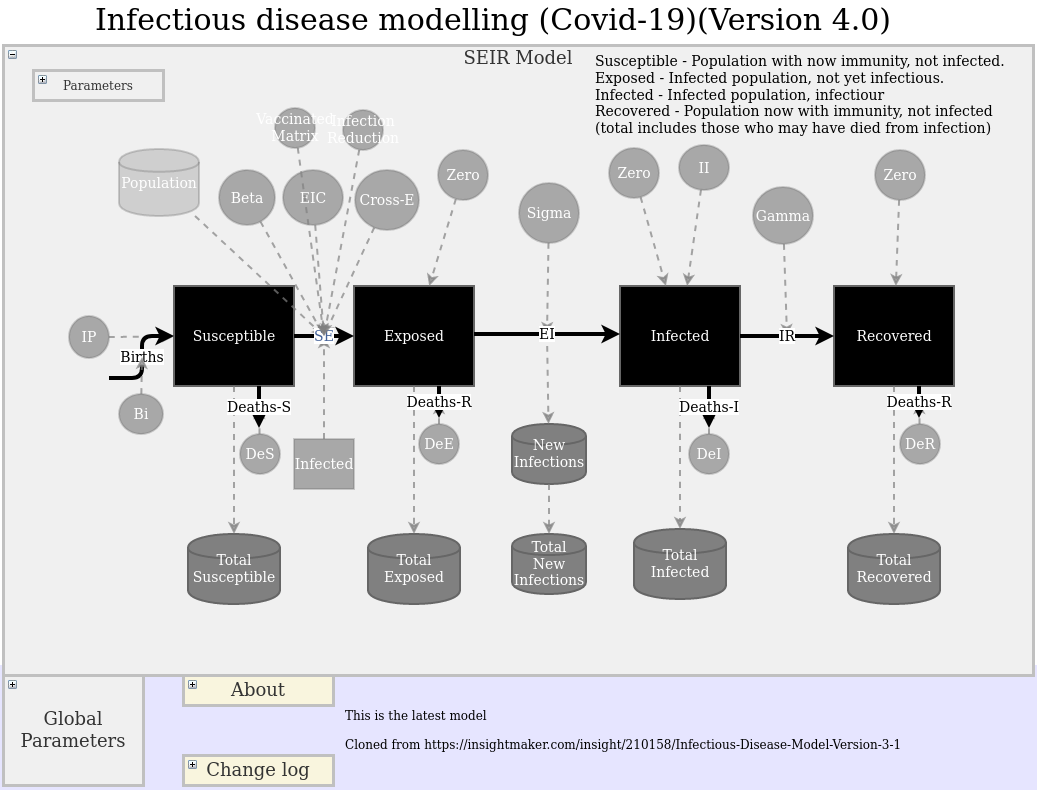
\includegraphics[width=\linewidth]{./figures/Covid19 SEIR Model.png}
	\caption[Double Diamond Design Process][6pt]{This is the interface of my copy of a Covid-19 SEIR (Susceptible-Exposed-Infected-Recovered) model developed for Public Health Dorset by (Source~\href{https://www.tanzo.org/}{Tanzo Creative} (Source~\href{https://insightmaker.com/insight/3aozzaFwITwi2Cn6ewR5Wj/Clone-of-Infectious-Disease-Model-Version-4-0}{Insight Maker}).}
	\label{fig:seir}
\end{figure*}


\section{Cardio-Vascular Disease Prevention}

\begin{description}
	\item[What?] We have constructed a systems model to simulate the impact of CVD prevention in local systems to support PHE colleagues in their renewed push for greater knowledge to action (Figure~\ref{fig:CVD}).
	\item[Why?] A systems model is a tool that can be used to capture knowledge and data into an interactive process of ‘what ifs’, that diverse groups of colleagues from an ICS can engage with each other to understand the behaviour of their local population and health system under various interventions.
	\item[So what?] Knowledge to action. Systems thinking and modelling provides a coherent pathway towards more informed decision-making through which there is improved shared-understanding of the challenges across the ICS. This will be the model used in our system modelling training course.
	\item[Insight?] Initial engagement with PHE staff in the CVD Prevention area indicates that they really appreciate what this type of modelling does and see a role for it within their programme.
\end{description}

\begin{figure*}[h]
	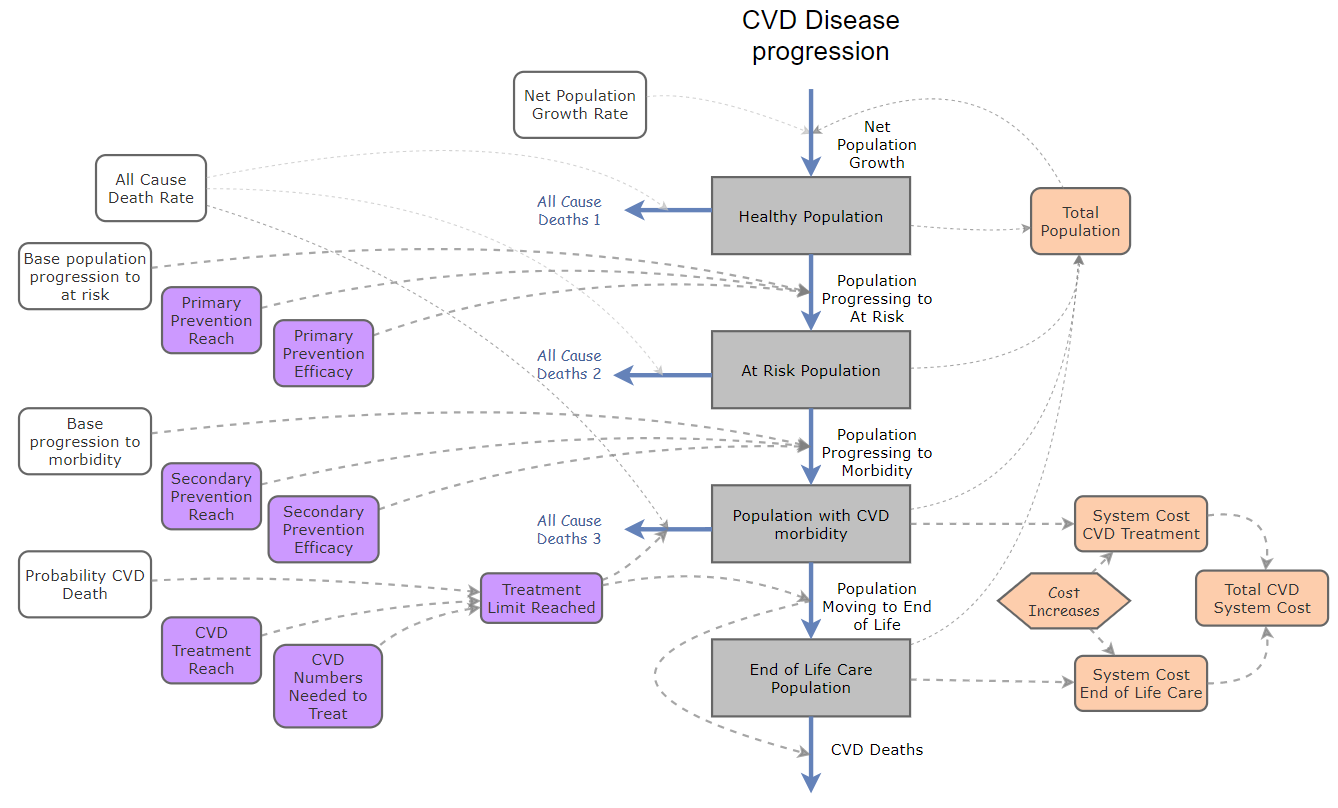
\includegraphics[width=\linewidth]{./figures/CVD Model.png}
	\caption[Double Diamond Design Process][6pt]{This is the interface of my copy of a CVD Prevention Model that I modified from a model developed by (Source: After~\href{https://www.tanzo.org/}{Tanzo Creative} (Source~\href{https://insightmaker.com/insight/1Oqiscp4ZdbYBaElk4Qq9W/CVD-System-Dynamics-Model-V1-1}{Insight Maker}).}
	\label{fig:CVD}
\end{figure*}